\documentclass[12pt,a4paper]{article}
\usepackage[utf8]{inputenc}
\usepackage[T1]{fontenc}
\usepackage{caption}
\usepackage{amsmath,amssymb,amsthm}
\usepackage{graphicx}
\usepackage{geometry}
\usepackage[hidelinks]{hyperref}
\usepackage{natbib}
\usepackage{booktabs}
\usepackage{titlesec}
\usepackage{float}
%\captionsetup[table]{skip=6pt}
\usepackage{setspace}
\usepackage{parskip}
\usepackage{tikz}
\usepackage{pgfplots}
\usepackage{tcolorbox}
\usetikzlibrary{positioning}
\renewcommand{\appendixname}{Appendix}
\hyphenation{Reproducibility}
\pgfplotsset{compat=1.18}
\setcounter{tocdepth}{3}
\setcounter{secnumdepth}{3}

\geometry{margin=1in}

% Section formatting
\titleformat{\section}
  {\normalfont\Large\bfseries}
  {\thesection}
  {1em}
  {}

\titlespacing*{\section}
  {0pt}
  {12pt}
  {6pt}

% Subsection formatting
\titleformat{\subsection}
  {\normalfont\large\bfseries}
  {\thesubsection}
  {1em}
  {}

\titlespacing*{\subsection}
  {0pt}
  {8pt}
  {4pt}

% Subsubsection formatting (added for better hierarchy)
\titleformat{\subsubsection}
  {\normalfont\normalsize\bfseries}
  {\thesubsubsection}
  {1em}
  {}

\titlespacing*{\subsubsection}
  {0pt}
  {6pt}
  {3pt}

\onehalfspacing

% Format abstract full page
\makeatletter
\renewenvironment{abstract}{
    \begin{center}
        {\large\bfseries \abstractname\vspace{-.5em}\vspace{0pt}}
    \end{center}
}{}
\makeatother

\title{MMLU and Cognitive Integrity: Clarifying Benchmark Interpretation in Regulatory Architectures}

\author{John H. Cragin \\
Independent Researcher \\
\href{mailto:john.cragin@outlook.com}{john.cragin@outlook.com} \\
ORCID: \href{https://orcid.org/0009-0001-5204-5732}{0009-0001-5204-5732}}

\date{\today}

\begin{document}

\sloppy

\maketitle

\begin{abstract}

Benchmarks like MMLU measure task-level optimization under uncertainty, but do not directly measure cognitive integrity—defined here as boundedness, coherence, and recoverability. Operationally, boundedness is assessed via drift (state variance across steps), coherence via an internal alignment score, and recoverability via hazard levels (instability risk). Intuitively, boundedness ensures the system stays within recoverable state space, coherence prevents internal alignment from degrading under load, and recoverability arrests instability escalation.

Using **SpiralBrain v3.0**, a Python-based neurosymbolic Regulatory Intelligence (RI) agent that runs locally on standard hardware and exposes internal regulatory metrics for inspection \cite{SpiralBrainV3,Cragin2026RI}, we show that low MMLU scores (20–36%) reflect intentional preservation of homeostasis rather than capability deficits. Internal integrity metrics instead indicate preserved boundedness and recovery behavior. Common misconceptions that benchmark performance implies cognitive competence are addressed, with implications for more careful benchmark usage. No claims of universality or superiority are made; conclusions are strictly constrained to observed behavior in SpiralBrain v3.0.

This work is situated within the Regulatory Intelligence (RI) paradigm \cite{Cragin2026RI}, which defines intelligence as the capacity for viability rather than calculation. Viability-first cognition prioritizes geometric homeostasis—maintaining bounded, coherent dynamics over time—over raw computational power. This connects directly to cognitive integrity: boundedness ensures state variance (drift) stays within recoverable limits, coherence maintains internal alignment (e.g., a normalized similarity between target and realized state vectors), and recoverability prevents instability escalation. Geometric homeostasis thus operationalizes integrity through elastic coupling mechanisms that adapt regulatory signals to environmental demands, e.g., coupling regulatory gains to state-distance in a latent geometry so that larger deviations induce stronger restorative forces. In this framework, MMLU serves as a structured stressor to probe regulatory mechanisms, with performance intentionally sacrificed to maintain homeostasis when hazard increases.

\end{abstract}

\section{Introduction}

Benchmarks play a central role in contemporary AI evaluation, providing standardized measures of system capabilities across diverse tasks. The Massive Multitask Language Understanding (MMLU) dataset, with its 15,908 questions spanning 57 academic subjects, is widely used to assess general knowledge, reasoning, and problem-solving in language models \cite{hendrycks2020measuring}. In practice, MMLU results are often interpreted as direct indicators of cognitive capability, where higher scores imply superior reasoning and lower scores suggest deficiencies.

This interpretation rests on an implicit assumption: that task performance equates to cognition. However, when benchmarks such as MMLU are repurposed as structured sources of uncertainty and contradiction rather than as capability rankings, this assumption breaks down. The purpose of this paper is to clarify MMLU interpretation in such contexts, using SpiralBrain v3.0 as an instrumented example to distinguish between task-level optimization and cognitive integrity under uncertainty. We make no claims of universality or superiority; all conclusions are constrained to empirically observed behavior in SpiralBrain.

\section{Related Work}

Benchmarks such as MMLU are widely used to evaluate task-level performance in language and reasoning systems \cite{hendrycks2020measuring}. However, prior work has noted that benchmark accuracy alone often fails to capture important dimensions of system behavior, particularly under distributional shift, ambiguity, or high-stakes deployment conditions. Several authors have argued that evaluation frameworks should move beyond aggregate accuracy toward behavioral testing, robustness analysis, and failure characterization \cite{raji2021beyond, ethayarajh2020utility}.

In the AI safety and interpretability literature, internal system properties—such as stability, sensitivity, and failure modes—are increasingly treated as first-class evaluation concerns rather than secondary diagnostics. Foundational work has emphasized that high task performance can coexist with undesirable internal behaviors, including brittleness, misgeneralization, and instability under stress \cite{amodei2016concrete, olah2018building}. These perspectives motivate evaluation approaches that explicitly instrument internal dynamics alongside external outcomes.

The present work builds on this line of reasoning by examining benchmark interpretation in the context of regulatory architectures. Rather than proposing a new benchmark or replacing existing ones, this paper clarifies how capability benchmarks such as MMLU should be interpreted when repurposed as structured stressors. Within the Regulatory Intelligence framework \cite{Cragin2026RI}, benchmarks are paired with internal integrity metrics—boundedness, coherence, and recoverability—to distinguish task-level optimization from stability-preserving regulation. This framing treats performance and integrity as complementary but orthogonal evaluation axes, particularly for systems designed to prioritize viability over accuracy.

\section{How MMLU Is Used in the Regulatory Intelligence Work}

In the Regulatory Intelligence work \cite{Cragin2026RI}, MMLU is employed not as a measure of capability but as a structured stressor to probe system stability under high-entropy conditions. The dataset's diverse questions across 57 academic subjects provide a controlled source of uncertainty and contradiction, allowing observation of how regulatory mechanisms respond to increasing cognitive load.

The protocol involves sampling all 57 subjects proportionally, with runs typically processing 1{,}000--2{,}000 questions to balance statistical reliability and computational cost. Mode selection and throttling are triggered when hazard exceeds predefined thresholds. For the experiments reported here, we use $H^{*} = 0.8$ and $H^{**} = 0.9$, activating restorative signals that downregulate high-convergence reasoning modules to prevent divergence, while maintaining coherence floors above $0.9$, where coherence is defined as
\[
c = \frac{\mathbf{v}_t \cdot \mathbf{v}_r}{\lVert \mathbf{v}_t \rVert \, \lVert \mathbf{v}_r \rVert}
\]
with $\mathbf{v}_t$ denoting the target state vector and $\mathbf{v}_r$ the realized state vector.

Experiments are conducted in a clean-slate, deterministic Python environment to ensure reproducibility and isolate internal physiology from external variables. Each run begins from identical initial conditions, with no persistent memory or cross-run learning, enabling falsification of regulatory behavior.

Dual measurement is used: both external task performance (MMLU accuracy) and internal cognitive physiology (metrics like coherence, hazard, and drift) are recorded simultaneously. This approach distinguishes stress testing—observing how the system maintains viability under load—from ranking systems by raw performance.

The goal is to observe regulatory throttling and homeostasis preservation, not to optimize scores. Lower MMLU performance is an intentional outcome of prioritizing stability over accuracy when hazard increases.

\section{MMLU in the H-Series Experimental Program}

The H-series is a staged experimental program designed to falsify specific regulatory hypotheses under increasing stress.

The Regulatory Intelligence work employs MMLU within the H-Series experimental program \cite{Cragin2026RI}, a systematic validation framework testing regulatory mechanisms under stress:

We operationalize these hypotheses by running MMLU stress tests under different regulatory configurations:

\begin{itemize}
\item \textbf{H3 (Structured Reasoning)}: Forces high-convergence logic, revealing coherence costs of intense reasoning; MMLU runs validate this by showing predictable throttling when coherence drops below 0.9, falsifying the hypothesis that high reasoning can be sustained without regulatory intervention.
\item \textbf{H4 (Elastic Coupling)}: Implements restorative signals to maintain coherence floors; if removed, integrity would collapse despite similar raw accuracy, indicating its necessity for stability.
\item \textbf{H5 (Cognitive Control Network)}: Enables autonomous mode selection based on hazard levels; MMLU experiments confirm this by demonstrating hazard-triggered shifts that preserve bounded dynamics.
\item \textbf{H6 (Long-Term Adaptation)}: Demonstrates 25.4\% drift reduction through regulatory optimization; this is evidenced by improved MMLU scores (up to 36.5\%) without integrity loss, validating adaptive regulatory efficacy.
\end{itemize}

Across H-series phases, MMLU performance ranges from 23.0\% to 36.5\%, with predictable regulatory responses: throttling activates when hazard rises, ensuring recoverable dynamics rather than divergence.

\section{Common Misconceptions About MMLU Results}

Common interpretations of MMLU results in regulatory architectures often lead to misconceptions about system capabilities.

\textbf{Misconception 1:} Low MMLU scores imply weak reasoning. In fact, scores in the 20–36\% range reflect intentional regulatory throttling to preserve homeostasis, not deficiencies in cognitive processing.

\textbf{Misconception 2:} Inconsistency or variability in performance implies confusion or collapse. Instead, it indicates elastic adaptation within runs, maintaining bounded dynamics without persistent learning.

\textbf{Misconception 3:} Non-learning systems are inherently disadvantaged on complex benchmarks. Regulatory architectures prioritize homeostasis over optimization, yielding lower scores but guaranteed stability.

These intuitions arise from optimization-centric paradigms but fail for systems designed for viability-first cognition. SpiralBrain v3.0 demonstrates that stability can be maintained even as accuracy is sacrificed.

\section{Cognitive Integrity vs Task Performance}

Cognitive integrity refers to a system's ability to maintain boundedness, coherence, and recoverability under stress, independent of task accuracy. In contrast, task performance measures correctness on specific objectives.

Accuracy is an insufficient proxy for integrity under uncertainty because it does not capture internal state. A system may achieve high performance while approaching instability, or low performance while preserving coherence.

Performance failure (e.g., incorrect answers) does not necessarily indicate cognitive failure (e.g., loss of bounded dynamics). Regulatory systems may deliberately fail tasks to maintain integrity.

Internal metrics like coherence (alignment), hazard (instability risk), and drift (state volatility) provide direct measures of integrity, revealing aspects invisible to performance alone.

While it is possible to tune architectures for both high accuracy and integrity, there exists a Pareto frontier where tradeoffs are inevitable under fixed regulatory designs. Our experiments probe a specific region of this frontier where integrity is explicitly prioritized, demonstrating that stability can be maintained even at lower performance levels. The baseline, enhanced reasoning, and H6 conditions can be read as three points on this frontier, with H6 moving closer to the region where both accuracy and integrity are acceptable.

\section{Illustrative Examples from SpiralBrain v3.0 MMLU Runs}

SpiralBrain v3.0's MMLU runs illustrate how low scores can coexist with preserved integrity \cite{Cragin2026RI}.

Example 1: In baseline conditions, MMLU performance reaches 23.3\%, with coherence remaining above 0.95 and homeostasis at 99.9\%, demonstrating that accuracy sacrifice preserves homeostasis. When hazard exceeded the threshold H* = 0.8, the control network downregulated high-convergence reasoning modules, coinciding with a measurable accuracy drop but keeping hazard below H** = 0.9.

Example 2: Under enhanced reasoning activation, scores improve to 29.9\% while maintaining bounded drift and low hazard, showing degradation without collapse. Here, elastic coupling signals were strengthened, allowing temporary accuracy gains without violating coherence floors.

Example 3: Across the H-series, performance ranges from 23.0\% to 36.5\%, with predictable failure modes: throttling activates when hazard rises, ensuring recoverable dynamics rather than divergence. In H6, optimized regulatory responses reduced drift by 25.4\%, enabling higher accuracy while preserving integrity.

These examples emphasize interpretation over achievement, highlighting how regulatory systems respond to stress.

\begin{figure}[H]
\centering
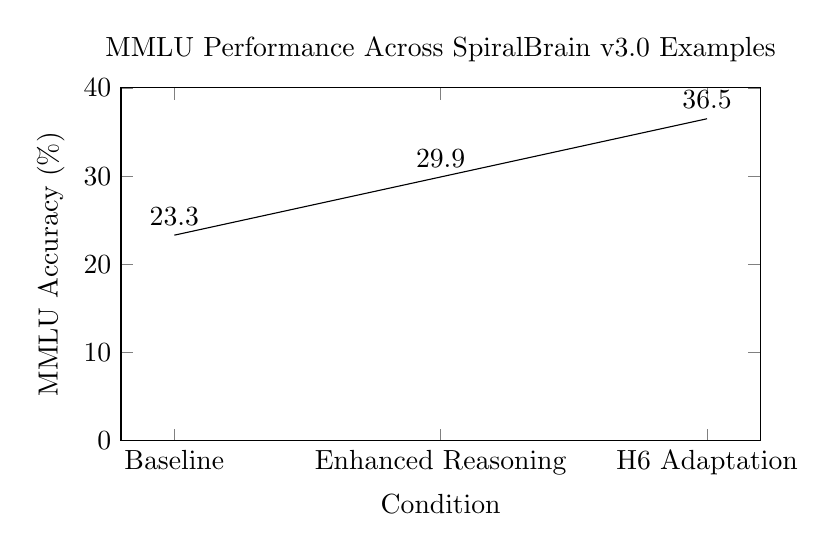
\begin{tikzpicture}
\begin{axis}[
    width=0.8\textwidth,
    height=0.5\textwidth,
    xlabel={Condition},
    ylabel={MMLU Accuracy (\%)},
    xtick={1,2,3},
    xticklabels={Baseline, Enhanced Reasoning, H6 Adaptation},
    ymin=0,
    ymax=40,
    bar width=0.4cm,
    nodes near coords,
    nodes near coords align={vertical},
    legend style={at={(0.5,-0.15)},anchor=north},
    title={MMLU Performance Across SpiralBrain v3.0 Examples}
]
\addplot[fill=blue!50] coordinates {(1,23.3) (2,29.9) (3,36.5)};
\end{axis}
\end{tikzpicture}
\caption{MMLU accuracy scores illustrating that accuracy changes track regulatory configuration rather than integrity loss. Baseline shows low scores with high integrity; enhanced reasoning improves accuracy while maintaining bounded dynamics; H6 adaptation achieves higher scores through optimized regulatory responses.}
\label{fig:mmlu_performance}
\end{figure}

\section{What MMLU Does Measure Well}

MMLU legitimately measures task-level performance in structured domains where answers are unambiguous, such as academic knowledge and reasoning.

It is appropriate for evaluating optimization-driven systems aiming for high accuracy, and useful for comparative ranking in those contexts.

This paper is not an attack on benchmarks; MMLU provides valuable signals when used for its intended purpose. However, overloading it with cognitive meaning beyond performance can mislead interpretations of regulatory systems.

\section{Implications for Benchmark Interpretation}

Overloading benchmarks with cognitive meaning risks misinterpreting regulatory systems, where low performance may reflect intentional homeostasis preservation rather than deficiency.

Internal instrumentation is essential for evaluating systems beyond external metrics, revealing coherence and hazard that performance alone obscures.

Regulatory systems should be evaluated differently: prioritize integrity metrics alongside accuracy, recognizing that stability-first designs may sacrifice performance for reliability.

This encourages more careful benchmark usage, distinguishing between optimization targets and stress tests.

Rather than rejecting benchmarks, this work advocates for orthogonalization: treating capability benchmarks (like MMLU for accuracy) and integrity instrumentation (for boundedness, coherence, recoverability) as complementary axes in a two-dimensional evaluation space. This allows systems to be assessed on both optimization potential and stability under stress, providing a more holistic view of AI architectures.

\section{Limitations}

This analysis is constrained to SpiralBrain v3.0 and its specific instrumentation; results may not generalize to other architectures without validation. To adapt this instrumentation to other systems, such as transformers, one could instrument attention layers for coherence analogs and monitor gradient norms for hazard proxies.

No claim of universality is made; the clarification applies only to regulatory systems similar to SpiralBrain v3.0.

No proposal for a replacement benchmark is offered; MMLU remains valuable for its intended uses.

All experimental results, analysis scripts, figure-generation pipelines, and logged outputs referenced in this study are publicly available in the SpiralBrain v3.0 repository \cite{SpiralBrainV3}.

An important open question is how to design standardized integrity benchmarks or shared instrumentation protocols across architectures, turning this limitation into a research agenda.

\section{Conclusion}

This paper clarifies how MMLU should be interpreted when used as a stressor in regulatory architectures, distinguishing task performance from cognitive integrity. Our results indicate that low MMLU scores in SpiralBrain v3.0 reflect stability-preserving regulatory responses rather than cognitive weakness, and that internal integrity metrics reveal information not captured by external accuracy alone. These findings suggest that benchmarks should be used cautiously to avoid overloading them with unwarranted cognitive meaning.

We recommend that future evaluations adopt dual measurement, reporting integrity metrics alongside performance on capability benchmarks, and we invite further work on standardized integrity instrumentation across architectures.

\bibliographystyle{plain}
\bibliography{references}

\end{document}